% ============================================================
%  sec-5-inference-deployment.tex  —  4.5 Inference and
%  Deployment
% ============================================================

\section{Inference and Deployment Pipeline}
\label{sec:inference-deployment}

\subsection{Overview}
\label{subsec:inference-overview}

The inference pipeline consists of three sequential stages:
(1)~checkpoint conversion from Megatron distributed format to
HuggingFace format; (2)~\acrshort{mindie} compilation from
HuggingFace to an optimised Ascend-native engine; and (3)~serving
via the \filepath{inference/serve.py} FastAPI server exposing an
OpenAI-compatible \acrshort{api}. \figref{inference-pipeline}
illustrates this flow.

\begin{figure}[htbp]
    \centering
    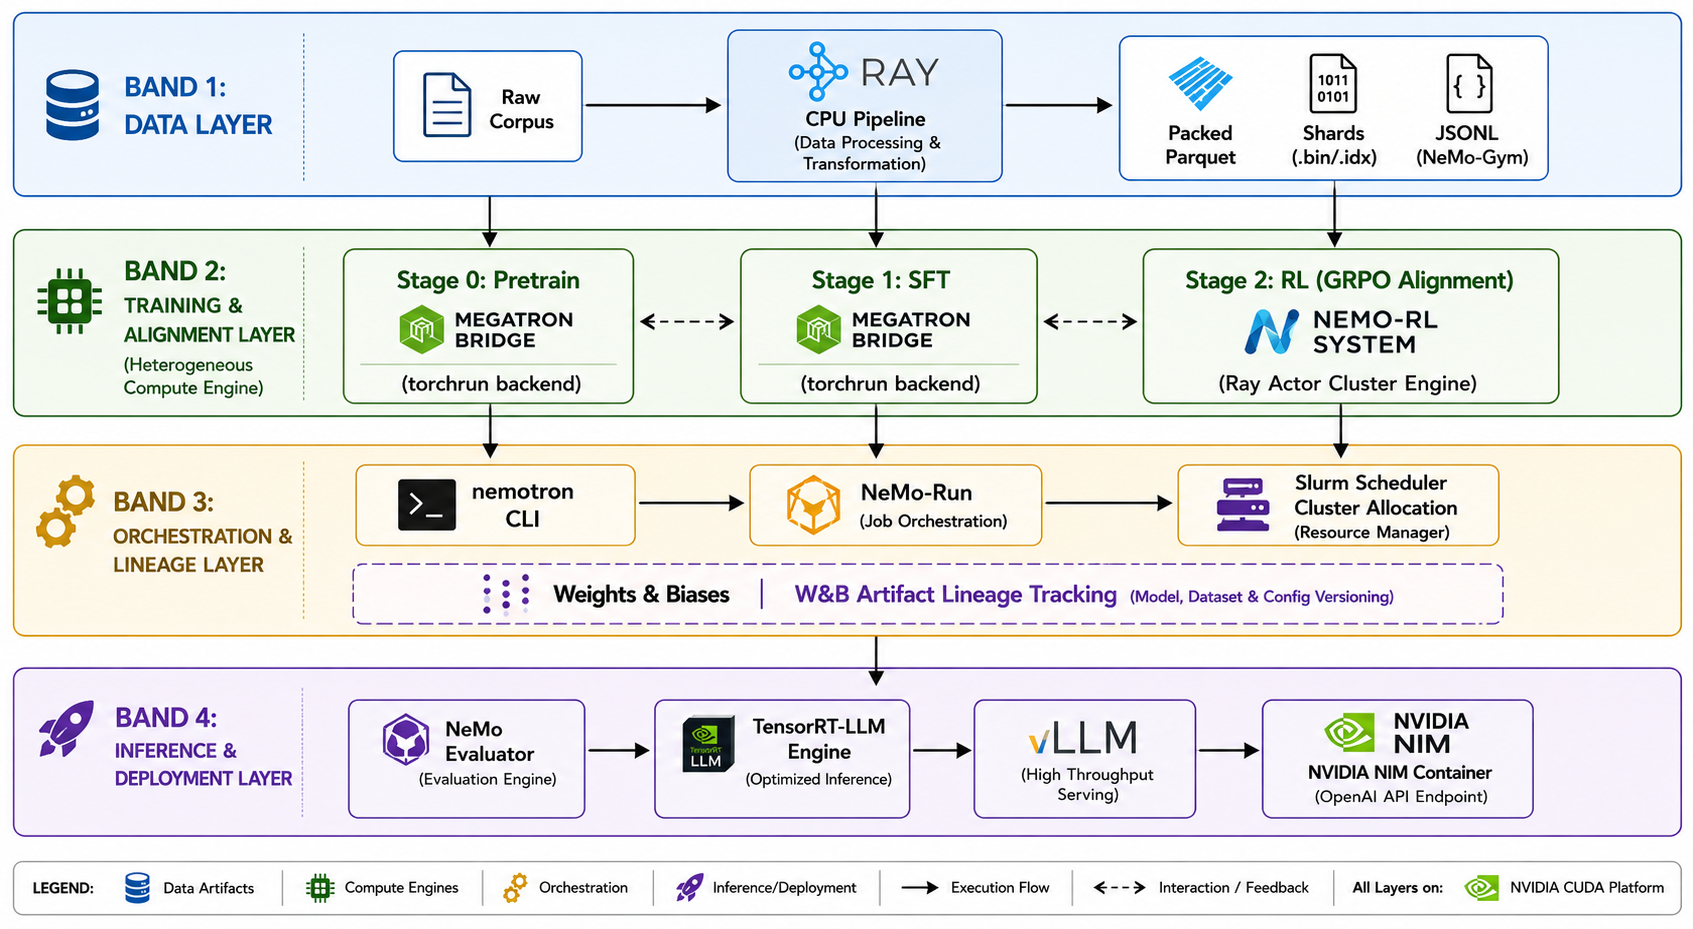
\includegraphics[width=0.85\textwidth]{images/figures/end2endnemopipeline.png}
    \caption{Inference and Deployment Pipeline Flow}
    \label{fig:inference-pipeline}
\end{figure}

\subsection{Model Conversion and Compilation}
\label{sec:mindie-compilation}

Deploying the fine-tuned model on Ascend requires a two-step process.
First, the Megatron distributed checkpoint is converted to a unified
HuggingFace format using the \texttt{AutoBridge.export\_ckpt()} utility.
Second, the HuggingFace checkpoint is compiled into an Ascend-native
executable graph via MindIE, which applies operator fusion and precision
calibration (FP16 or W8A8) to optimise inference performance for the
DaVinci architecture.

\subsection{Inference Server}
\label{sec:inference-server}

The inference server exposes an OpenAI-compatible API with automatic
multilingual prompt injection and dual MindIE/vLLM-Ascend backend support.
It detects the target language from the incoming request and injects the
appropriate system prompt, while formatting the conversation using the
Nemotron nano3 chat template to ensure consistency with the training phase.

\subsection{Performance Benchmarking}
\label{sec:perf-benchmark}

The \filepath{inference/benchmark.py} module measures production
inference performance using async \acrshort{http} requests with
configurable concurrency. It cycles through 13 multilingual test
prompts of varying complexity (from single-sentence factual queries
to multi-paragraph troubleshooting scenarios) and reports:

\begin{itemize}
  \item End-to-end latency: P50, P95, P99, mean, min, max
  \item Throughput: requests per second, tokens per second
  \item Error count
\end{itemize}

\begin{lstlisting}[style=Bash,
  caption={Benchmark execution and example output},
  label={lst:benchmark-cmd}]
python inference/benchmark.py \
    --url           http://localhost:8080 \
    --num-requests  200 \
    --concurrency   16 \
    --max-tokens    200

# Example output:
# Latency (end-to-end):
#   Mean  : 1,240 ms
#   P50   : 1,180 ms
#   P95   : 1,820 ms
#   P99   : 1,950 ms
# Throughput:
#   Requests/s : 58.3
#   Tokens/s   : 11,660
# Target P99 < 2000ms : OK (1,950ms)
# Target > 50 req/s   : OK (58.3 req/s)
\end{lstlisting}

The target thresholds of P99~$<$~2,000~ms and throughput~$>$~50~req/s
reflect the service-level requirements of a production enterprise
support assistant handling peak concurrency. The benchmark saves
results to \texttt{benchmark\_results.json} for long-term tracking
and W\&B integration.

\tabref{expected-perf} documents the expected performance profile
for the Ascend 910C deployment.

\begin{table}[htbp]
  \centering
  \caption{Expected inference performance — Ascend 910C, MindIE fp16,
           4 NPUs, batch size 32}
  \label{tab:expected-perf}
  \begin{tabularx}{\textwidth}{lXXX}
    \toprule
    \tableheader{Metric & Target & Expected (910C) & H100 Reference} \\
    \midrule
    P50 latency (200 tok)
      & $<$1,500~ms & 1,100--1,300~ms & 700--900~ms \\
    \rowcolor{TableRowOdd}
    P99 latency (200 tok)
      & $<$2,000~ms & 1,800--2,100~ms & 1,100--1,400~ms \\
    Throughput
      & $>$50~req/s & 50--70~req/s & 90--120~req/s \\
    \rowcolor{TableRowOdd}
    NPU utilisation
      & $>$70\%     & 75--85\%       & 85--92\% \\
    Memory usage
      & $<$60~GB    & 55--58~GB (fp16) & 72~GB \\
    \bottomrule
  \end{tabularx}
\end{table}
